% Guide de maîtrise du projet (pour la soutenance et les questions du jury).
% Compilation :  cd report && latexmk -pdf guide_projet.tex
\documentclass[11pt,a4paper]{article}
\usepackage[utf8]{inputenc}
\usepackage[T1]{fontenc}
\usepackage[french]{babel}
\usepackage{lmodern}
\usepackage[margin=2.3cm]{geometry}
\usepackage{amsmath,amssymb}
\usepackage{graphicx}
\usepackage{booktabs}
\usepackage{xcolor}
\usepackage{enumitem}
\usepackage[section]{placeins}
\usepackage{tikz}
\usetikzlibrary{arrows.meta,positioning}
\usepackage[most]{tcolorbox}
\usepackage{hyperref}
\hypersetup{colorlinks=true,linkcolor=blue!50!black,urlcolor=blue!50!black}
\graphicspath{{figures/}}

\newtcolorbox{intuition}{breakable,colback=blue!4,colframe=blue!45!black,title=L'idée simple,fonttitle=\bfseries}
\newtcolorbox{exemple}{breakable,colback=green!4,colframe=green!35!black,title=Exemple chiffré,fonttitle=\bfseries}
\newtcolorbox{piege}{breakable,colback=red!4,colframe=red!55!black,title=Pièges classiques (questions du jury),fonttitle=\bfseries}
\newtcolorbox{resultat}{breakable,colback=orange!5,colframe=orange!60!black,title=Ce que nous avons mesuré,fonttitle=\bfseries}
\newtcolorbox{retenir}{breakable,colback=gray!6,colframe=gray!60!black,title=À retenir,fonttitle=\bfseries}

\newcommand{\T}{^{\mathsf T}}
\newcommand{\x}{\mathbf{x}}
\newcommand{\X}{\mathbf{X}}

\title{\textbf{Les vidéos générées respectent-elles la géométrie d'une caméra ?}\\[4pt]
\large Guide de maîtrise du projet, de l'intuition à la rigueur\\
CSC\_51073\_EP, Image Analysis and Computer Vision, École polytechnique}
\author{Projet de Khalil et Ahmed}
\date{Novembre 2026}

\sloppy
\begin{document}
\maketitle

\noindent Ce guide explique tout le projet de manière autonome : le problème, chaque méthode, ses
équations, ce que nous avons mesuré, et les questions qu'un jury peut poser. Tous les chiffres
viennent de l'exécution de notre code (dossiers \texttt{results/latest},
\texttt{results/latest\_vifbench}, \texttt{results/inspect}, tests de \texttt{tests/}). Quand un
résultat a été invalidé par une vérification ultérieure, le guide le dit.

\tableofcontents
\newpage

%=====================================================================================
\section{La big picture et l'intuition fondamentale}
%=====================================================================================

\subsection{À quoi sert ce projet dans le monde réel ?}

Une vraie vidéo est une \textbf{mesure physique}. La lumière d'une scène 3D traverse un objectif,
frappe un capteur, puis l'image est traitée et compressée. Chaque étape impose des contraintes
mathématiques que la vidéo respecte \emph{automatiquement}, sans que personne ne s'en occupe :
\begin{itemize}
  \item deux images d'une scène immobile vérifient la contrainte épipolaire $\x^{\prime\mathsf{T}} F\x=0$ ;
  \item un point vu dans deux images a une position 3D, donc une position \emph{prévisible} dans une
        troisième image ;
  \item des droites parallèles en 3D se coupent en un seul point de fuite, et ces directions 3D
        tournent toutes ensemble quand la caméra tourne ;
  \item le mouvement des pixels (flot optique) est entièrement déterminé par la profondeur et par
        le mouvement de la caméra ;
  \item le bruit du capteur a un spectre lisse, sans pics périodiques.
\end{itemize}

Un générateur vidéo (Sora, Veo, Kling, Wan\ldots) n'a pas de caméra ni de scène 3D. Il apprend à
produire des images \emph{qui ressemblent} à des vidéos. La question du projet est donc :
\begin{center}
\emph{Les vidéos générées respectent-elles, à la précision de nos instruments, les contraintes
qu'une vraie caméra respecte toujours ?}
\end{center}

Le but n'est \textbf{pas} de construire le meilleur détecteur possible. Le but est d'\textbf{appliquer les
méthodes du cours} (et une méthode hors cours, V5) comme des instruments de mesure, puis de voir
honnêtement ce qu'ils mesurent.

\subsection{Analogie maîtresse : l'interrogatoire de témoins}

Imagine un enquêteur qui interroge un témoin.
\begin{itemize}
  \item Chaque phrase du témoin est plausible. De même, chaque frame d'une vidéo générée est
        une image réaliste. Regarder une frame seule ne suffit pas.
  \item L'enquêteur \textbf{recoupe} : la phrase de 14\,h est-elle compatible avec celle de 15\,h ?
        C'est le test épipolaire entre deux frames (V1).
  \item Il recoupe trois déclarations : si le témoin était à A à 14\,h et à B à 15\,h, il ne pouvait
        être qu'à C à 16\,h. C'est le test à trois vues de la Session 7 : deux vues fixent un point
        3D, la troisième doit le voir exactement là où il est prévu.
  \item Il vérifie l'alibi avec un élément extérieur : la profondeur vue par un réseau de neurones
        doit expliquer le mouvement des pixels (V5).
  \item Il écoute la voix : un enregistrement trafiqué a un bruit de fond anormal. C'est le spectre
        du bruit (I1).
\end{itemize}
Deux pièges de l'enquêteur sont aussi les nôtres :
\begin{itemize}
  \item un témoin \textbf{nerveux} (qui bafouille) n'est pas forcément un menteur. Une vidéo générée
        un peu floue donne des points moins bien localisés, donc des erreurs plus grandes, sans
        aucune faute de 3D. C'est le \textbf{piège du rendu} ;
  \item un témoin qui \textbf{dit peu de choses} se contredit peu. Une vidéo qui bouge peu donne des
        erreurs petites. C'est le \textbf{piège du mouvement}.
\end{itemize}
Tout le travail sérieux du projet consiste à séparer \og ment \fg{} de \og bafouille \fg{} et de
\og parle peu \fg.

\subsection{Architecture du projet : le fil rouge}

Chaque étage de la chaîne physique donne une contrainte, chaque contrainte donne un test, chaque
test vient d'une session du cours.

\begin{table}[!htbp]
\centering\small
\resizebox{\linewidth}{!}{\begin{tabular}{@{}lllll@{}}
\toprule
Étage physique & Contrainte & Test & Session & Fichier \\
\midrule
Scène 3D rigide, 2 vues & $\x^{\prime\mathsf{T}} F\x=0$ & V1 paires & 3, 4 & \texttt{video\_epipolar.py} \\
Scène 3D rigide, 3 vues & position prévue en vue 3 & V1 trois vues & 7 & \texttt{multiview.py} \\
Projection perspective & droites parallèles $\to$ 1 point de fuite & I2 & 1--4 & \texttt{image\_perspective.py} \\
Continuité temporelle & texture stable après compensation & V3 & 3, 6 & \texttt{video\_temporal.py} \\
Capteur et traitement & spectre du bruit lisse & I1 & 1--2 & \texttt{image\_frequency.py} \\
Flot = f(profondeur, caméra) & modèle de flot rigide & V5 & hors cours & \texttt{video\_rigidflow.py} \\
Apparence (référence) & -- & CLIP & 5 & \texttt{baseline\_clip.py} \\
\bottomrule
\end{tabular}}
\end{table}

\begin{figure}[!htbp]
\centering
\begin{tikzpicture}[node distance=0.55cm and 0.5cm, every node/.style={font=\small},
  box/.style={draw,rounded corners,fill=blue!6,align=center,minimum height=0.9cm,text width=2.5cm},
  arr/.style={-{Latex},thick}]
\node[box] (data) {Clips réels et générés\\ (16 nôtres, 3160 ViF-Bench)};
\node[box,right=of data] (norm) {Normalisation\\ identique (fps, taille, CRF)};
\node[box,right=of norm] (feat) {Mesures physiques\\ V1, I2, V3, I1, V5};
\node[box,right=of feat] (cmp) {Comparaison à mouvement égal};
\node[box,below=of cmp] (clf) {Classifieurs, CV par scène, vs CLIP};
\node[box,below=of feat] (out) {Rapport HTML, démo vidéo, rapport \LaTeX};
\draw[arr] (data)--(norm); \draw[arr] (norm)--(feat); \draw[arr] (feat)--(cmp);
\draw[arr] (feat.south east)--(clf.west); \draw[arr] (cmp)--(clf); \draw[arr] (clf)--(out);
\end{tikzpicture}
\caption{Pipeline (\texttt{python -m src.run}). Les algorithmes centraux (RANSAC, 8 points,
DLT, Sampson, triangulation, points de fuite, ajustement du flot rigide) sont écrits par nous en numpy.}
\end{figure}

\subsection{Le message en cinq phrases (à savoir dire par cœur)}
\begin{enumerate}
  \item Nos instruments géométriques fonctionnent : sur des clips synthétiques à géométrie connue,
        ils détectent une scène qui se déforme et ignorent un simple flou.
  \item La distance de Sampson brute mesure surtout le \textbf{rendu} (précision des points), pas la
        3D : notre contrôle sur vid4 le prouve (même écart réel/généré dans la partie copiée du réel).
  \item À précision et mouvement égaux, les vidéos générées sont \textbf{localement aussi rigides}
        que les vraies sur des fenêtres de quelques secondes ; l'effet de \og croissance \fg{} vu
        sur ViF-Bench disparaît quand on corrige le mouvement et le plancher de bruit.
  \item Ce qui sépare réel et généré sur ViF-Bench, c'est l'apparence (CLIP, AUC 0,77) bien plus
        que la physique (AUC 0,65) ; les deux ne se recoupent pas totalement (fusion tardive +0,018).
  \item Les indices physiques restent utiles comme \textbf{explications} : ils disent \emph{où} et
        \emph{comment} une vidéo s'écarte d'une caméra (cas du drone vid6, cartes de V5).
\end{enumerate}

%=====================================================================================
\section{Roadmap d'apprentissage stratégique}
%=====================================================================================

\subsection{Ordre optimal}
\begin{enumerate}
  \item \textbf{Coordonnées homogènes et projection} $\x \sim K[R\,|\,t]\X$. Tout le reste en dépend.
  \item \textbf{RANSAC}. Toutes nos estimations sont robustes ; comprendre seuil, inliers et nombre
        de tirages.
  \item \textbf{Appariement SIFT} (ratio de Lowe, vérification mutuelle).
  \item \textbf{Matrice fondamentale} : contrainte, 8 points normalisé, rang 2, distance de Sampson.
  \item \textbf{Homographie} : quand $F$ ne dit rien (rotation pure, scène plane), parallaxe.
  \item \textbf{Les confondants} : rendu, mouvement, plancher de bruit. C'est le cœur scientifique.
  \item \textbf{Test à trois vues} (Session 7) : caméras depuis $F$, triangulation, DLT de caméra,
        croissance de l'erreur.
  \item \textbf{Points de fuite} (I2) puis \textbf{flot optique} (V3) puis \textbf{Fourier} (I1).
  \item \textbf{Évaluation} : AUC, validation croisée par scène, générateur jamais vu, fusion.
  \item \textbf{V5} : modèle de flot rigide avec profondeur apprise (hors cours).
\end{enumerate}

\subsection{Les 20\,\% qui débloquent les 80\,\%}
\begin{enumerate}
  \item \textbf{Un résidu géométrique mélange trois choses} : l'erreur de géométrie (ce qu'on cherche),
        le bruit de localisation des points (rendu) et la quantité de mouvement. Tant que ceci n'est
        pas clair, aucun résultat n'est interprétable. Déblocage : se demander pour chaque chiffre
        \og si la vidéo était juste plus floue, ce chiffre changerait-il ? \fg.
  \item \textbf{Les cas dégénérés} : sans translation de la caméra, $F$ n'est pas définie de façon
        utile (tout est expliqué par une homographie). Déblocage : la parallaxe et \texttt{h\_cover}.
  \item \textbf{L'ambiguïté projective} : sans calibration, on reconstruit la scène à une
        transformation projective près. Le test à trois vues marche quand même, car il compare des
        \emph{positions d'image}, invariantes à cette ambiguïté.
  \item \textbf{La fuite de données} : si une scène est à la fois en apprentissage et en test, le
        classifieur reconnaît le contenu. Déblocage : découpage par \texttt{scene\_id}.
  \item \textbf{L'AUC} : probabilité qu'une vidéo générée tirée au hasard ait un score plus haut
        qu'une vraie. 0,5 = hasard. Elle ne dépend d'aucun seuil.
\end{enumerate}

%=====================================================================================
\section{Le projet complet : intuition et rigueur, méthode par méthode}
%=====================================================================================

\subsection{Fondations : géométrie projective}

\begin{intuition}
Une caméra écrase le monde 3D sur un plan. Les coordonnées homogènes ajoutent un 1 aux points pour
que cette opération (et les translations) devienne une simple multiplication de matrices. Deux
vecteurs proportionnels représentent le même point.
\end{intuition}

\paragraph{Formalisme.}
Point image $\x=(u,v,1)\T$, point 3D $\X=(X,Y,Z,1)\T$, projection
\[ \lambda\,\x = P\X,\qquad P = K\,[R\,|\,t],\qquad
K=\begin{pmatrix} f & 0 & c_x\\ 0 & f & c_y\\ 0&0&1\end{pmatrix}. \]
\begin{itemize}
  \item $K$ (intrinsèques) : $f$ focale en pixels (plus grande $f$ = champ plus étroit), $(c_x,c_y)$
        point principal ;
  \item $R,t$ (extrinsèques) : rotation et translation monde $\to$ caméra ;
  \item $\lambda$ : profondeur du point, perdue par la projection.
\end{itemize}
Droite passant par deux points : $\boldsymbol\ell=\x_1\times\x_2$. Intersection de deux droites :
$\x=\boldsymbol\ell_1\times\boldsymbol\ell_2$. Un point à l'infini a une troisième coordonnée nulle
(c'est ainsi qu'un point de fuite \og à l'infini \fg{} reste manipulable).

\subsection{RANSAC : estimer malgré les faux appariements}

\begin{intuition}
Parmi des centaines d'appariements, 10 à 50\,\% sont faux. Une moyenne serait ruinée. RANSAC tire un
petit échantillon minimal, ajuste un modèle, compte combien de données sont d'accord (les
\emph{inliers}), recommence, et garde le modèle le plus soutenu.
\end{intuition}

\paragraph{Formalisme} (\texttt{src/geometry/ransac.py}, cours EP3).
\begin{enumerate}
  \item tirer $s$ données (taille minimale : 8 pour $F$, 4 pour $H$, 6 pour une caméra, 2 pour un
        point de fuite) ;
  \item ajuster le modèle, calculer le résidu $r_i$ de chaque donnée, inliers si $r_i<\tau$ ;
  \item garder le meilleur modèle ; mettre à jour le nombre de tirages nécessaires
  \[ N=\left\lceil\frac{\log(1-p)}{\log\bigl(1-(1-e)^s\bigr)}\right\rceil \]
        où $p$ est la probabilité voulue d'avoir au moins un échantillon sans faux (0,99), $e$ la
        part de faux estimée par le meilleur modèle ;
  \item réajuster par moindres carrés sur tous les inliers, recalculer les inliers, répéter jusqu'à
        stabilité.
\end{enumerate}
Rôle des termes : si $e$ augmente, $(1-e)^s$ s'effondre et $N$ explose ; si $s$ augmente, même effet.
C'est pourquoi on choisit toujours l'échantillon \emph{minimal}. Le seuil $\tau$ fixe ce qu'on appelle
\og d'accord \fg{} : trop petit, les vrais appariements bruités sont rejetés ; trop grand, les faux
passent.

\begin{exemple}
$F$ avec $e=0{,}3$, $s=8$, $p=0{,}99$ : $(0{,}7)^8=0{,}0576$, $\log(1-0{,}0576)=-0{,}0594$,
$\log(0{,}01)=-4{,}605$, donc $N=\lceil 77{,}6\rceil = 78$ tirages. Si $e=0{,}5$ :
$0{,}5^8=0{,}0039$, $N=1177$. D'où notre plafond de 5000 tirages et l'importance d'un bon appariement.
\end{exemple}

\subsection{Appariement de points : SIFT, ratio de Lowe, vérification mutuelle}

\begin{intuition}
On cherche le même détail physique dans deux images. SIFT décrit chaque point par un histogramme
d'orientations de gradients (128 nombres), stable aux changements d'échelle et de rotation. Un
appariement est gardé s'il est nettement meilleur que le second choix, et réciproque.
\end{intuition}

\paragraph{Formalisme.} Pour un descripteur $\mathbf d$ de l'image 1, $d_1$ et $d_2$ sont les distances
à ses deux plus proches voisins dans l'image 2. On garde si $d_1<0{,}75\,d_2$ (ratio de Lowe, EP3)
\emph{et} si le point de l'image 1 est aussi le plus proche voisin de son partenaire (mutuel). Les
points sont répartis sur une grille $8\times8$ (même quota par case) pour que la géométrie soit
contrainte sur toute l'image et pas seulement sur une zone texturée.

\begin{piege}
\begin{itemize}
  \item Textures répétitives (grillages, carrelage) : faux appariements cohérents entre eux, que
        RANSAC peut accepter. Le ratio test strict les limite.
  \item Le nombre d'appariements dépend du \emph{rendu} (texture, netteté). Une feature \og nombre de
        points \fg{} mesure l'apparence, pas la 3D. Nous l'avons classée dans le groupe \og matching \fg.
\end{itemize}
\end{piege}

\subsection{La matrice fondamentale et la distance de Sampson (V1, Sessions 3--4)}

\begin{intuition}
Si la caméra bouge dans une scène immobile, un point de l'image 1 ne peut apparaître, dans l'image 2,
que sur une droite précise : la droite épipolaire. Une seule matrice $3\times 3$, $F$, encode ces
droites pour tous les points. Une vidéo réelle de scène statique doit donc s'expliquer par une $F$.
\end{intuition}

\paragraph{Formalisme} (\texttt{src/geometry/fundamental.py}, \texttt{errors.py}).
\[ \x^{\prime\mathsf{T}} F\,\x = 0,\qquad \boldsymbol\ell' = F\x \text{ (droite épipolaire dans l'image 2)}. \]
$F$ a 9 coefficients, définie à l'échelle près, et $\det F=0$ (rang 2) : 7 degrés de liberté.

\emph{Algorithme des 8 points.} Chaque appariement $\bigl((u,v),(u',v')\bigr)$ donne une ligne
\[ \bigl[u u',\ v u',\ u',\ u v',\ v v',\ v',\ u,\ v,\ 1\bigr]\cdot \mathbf f = 0 . \]
Avec $N\ge 8$ lignes, on empile $A\mathbf f=0$ et on prend le vecteur singulier de $A$ associé à la
plus petite valeur singulière. On force ensuite le rang 2 : $F=U\,\mathrm{diag}(\sigma_1,\sigma_2,0)\,V\T$.

\emph{Normalisation.} Les coordonnées en pixels (de l'ordre de 1000) donnent des colonnes de $A$
d'échelles très différentes ($uu'\sim10^6$, $1$) : la SVD est mal conditionnée. On ramène les points
autour de $[-1,1]$ ($\hat\x=T\x$), on estime $\hat F$, puis $F=T^{\prime\mathsf{T}}\hat F\,T$ (EP4 slide 104).

\emph{Distance de Sampson} (H\&Z éq. 11.9), notre résidu :
\[ d_S=\frac{|\x^{\prime\mathsf{T}} F\x|}{\sqrt{(F\x)_1^2+(F\x)_2^2+(F\T\x')_1^2+(F\T\x')_2^2}} . \]
Rôle des termes : le numérateur est l'erreur \emph{algébrique} (sans unité) ; le dénominateur est la
norme du gradient de cette erreur par rapport aux quatre coordonnées. Le quotient approxime au premier
ordre la plus petite correction (en pixels) des deux points qui rendrait l'appariement exactement
cohérent. C'est donc une distance en pixels, comparable entre vidéos.

\begin{exemple}
Caméra en translation horizontale pure : $F=\begin{pmatrix}0&0&0\\0&0&-1\\0&1&0\end{pmatrix}$, et
la contrainte devient $v=v'$ (les points restent sur la même ligne). Pour $\x=(100,50)$,
$\x'=(130,51)$ : $F\x=(0,-1,50)\T$, $F\T\x'=(0,1,-51)\T$, numérateur $|50-51|=1$, dénominateur
$\sqrt{0+1+0+1}=\sqrt2$, donc $d_S=0{,}71$ px. L'écart vertical de 1 px est partagé entre les deux
points : chacun bouge d'environ 0,5 px dans la meilleure correction.
\end{exemple}

\begin{piege}
\begin{itemize}
  \item \textbf{Sampson mesure aussi le rendu.} Un point mal localisé (flou, texture qui bouge) donne un
        grand $d_S$ même dans une scène parfaitement rigide. Synthétique : flou $\sigma=1{,}5$ fait
        passer Sampson de 0,090 à 0,127 px (+41\,\%) sans toucher à la géométrie.
  \item \textbf{Une contrainte de droite, pas de point.} Un point qui glisse le long de sa droite
        épipolaire (profondeur qui change) n'est pas vu par $F$. D'où le test à trois vues.
  \item \textbf{Rotation pure ou scène plane} : une homographie explique tout, $F$ n'est pas
        identifiable. Il faut mesurer la parallaxe.
  \item \textbf{Objets mobiles} : une vraie vidéo avec des passants ne vérifie pas non plus une seule $F$.
\end{itemize}
\end{piege}

\subsection{L'homographie, la couverture et la parallaxe}

\begin{intuition}
Si la caméra ne fait que tourner, ou si la scène est plate ou très lointaine, les deux images sont
reliées par une simple déformation projective du plan : une homographie $H$ (c'est le principe des
panoramas du TP 3). Ce qu'une homographie \emph{ne peut pas} expliquer, c'est la parallaxe : le
décalage relatif entre objets proches et lointains, signature de la translation et de la 3D.
\end{intuition}

\paragraph{Formalisme.} $\x'\sim H\x$, $H$ $3\times3$ à 8 degrés de liberté, estimée par DLT normalisée
(4 points minimum, 2 équations par point) dans RANSAC avec l'erreur de transfert symétrique
$\tfrac12\bigl(\|\x'-H\x\|+\|\x-H^{-1}\x'\|\bigr)$. Nous en tirons :
\begin{itemize}
  \item \texttt{h\_cover} : part des inliers de $F$ aussi expliqués par $H$. Proche de 1 : la paire
        est dégénérée, $F$ ne dit presque rien ;
  \item \texttt{parallax\_px} : erreur de transfert médiane des inliers de $F$ sous $H$, en pixels.
\end{itemize}

\subsection{Comparer à mouvement égal : le premier confondant}

\begin{intuition}
Toutes les erreurs grandissent avec le mouvement entre deux frames (points plus déformés, plus
d'occlusions). Or les vidéos générées bougent souvent \emph{moins}. Comparer à écart temporel égal
avantage donc injustement les vidéos générées.
\end{intuition}

\paragraph{Méthode} (\texttt{src/eval/compare.py}). Pour chaque scène, on prend la plage de mouvement
image (flot médian des appariements, en px) commune à toutes ses vidéos (entre leurs percentiles 10 et
90), on la découpe en 5 intervalles logarithmiques, et on compare les médianes de Sampson dans les
\emph{mêmes} intervalles. Le rapport généré/réel est la moyenne géométrique sur les intervalles communs.

\paragraph{Le contrôle de vid4 : la preuve que Sampson mesure le rendu.} Les deux versions générées de
vid4 ont reçu les 2 premières secondes du clip réel. Dans cette fenêtre, la géométrie est \emph{celle
du réel} (le générateur l'a recopiée), seul le rendu change.
\begin{resultat}
Rapport de Sampson généré/réel à mouvement égal : 1,33 et 1,31 sur tout le clip, \textbf{1,30 et 1,29
dans la fenêtre copiée}. L'écart est le même là où la géométrie est vraie : il vient du rendu, pas de
la 3D. La croissance trois vues dans la fenêtre copiée vaut 0,99 et 0,91 fois celle du réel.
\end{resultat}

\subsection{Le test à trois vues (V1, Session 7)}

\begin{intuition}
Deux vues suffisent à trianguler un point 3D. Une troisième vue doit alors voir ce point exactement
là où la géométrie le prévoit : la contrainte devient un \emph{point}, plus une droite. Et si la scène
dérive lentement, l'erreur grandit avec l'écart entre les vues. Le rapport entre l'erreur à grand écart
et l'erreur à petit écart (la \emph{croissance}) devrait ignorer le rendu, qui gonfle les deux pareil.
\end{intuition}

\paragraph{Formalisme} (\texttt{src/geometry/multiview.py}), sur des triplets de frames $(t,t+k,t+2k)$.
\begin{enumerate}
  \item \textbf{Caméras depuis $F$} (H\&Z résultat 9.14) :
  \[ P_1=[I\,|\,\mathbf 0],\qquad P_2=\bigl[[\mathbf e']_\times F\ \big|\ \mathbf e'\bigr],\qquad F\T\mathbf e'=0 .\]
  $\mathbf e'$ est l'épipole de l'image 2 (vecteur singulier gauche de $F$) et $[\mathbf e']_\times$
  la matrice du produit vectoriel. Reconstruction \emph{projective} : aucune calibration $K$ n'est
  nécessaire.
  \item \textbf{Triangulation linéaire (DLT)} : de $\lambda\x=P\X$ on tire, pour chaque vue,
  $(x\,\mathbf p_3\T-\mathbf p_1\T)\X=0$ et $(y\,\mathbf p_3\T-\mathbf p_2\T)\X=0$ ; 4 équations,
  $\X$ = vecteur singulier de plus petite valeur singulière.
  \item \textbf{Calibration de la troisième caméra par DLT} : $M$ ($3\times4$, 11 degrés de liberté),
  2 équations par correspondance 3D--2D, donc au moins 6 points, estimée dans un RANSAC
  (échantillons de 6, seuil 2 px sur l'erreur de reprojection).
  \item \textbf{Erreur de reprojection} dans la vue 3 : $e=\|\x_3-\pi(M\X)\|$, médiane sur les points.
  \item \textbf{Croissance} : $g=\dfrac{e(k_{\max})}{e(k_{\min})}$, avec $k\in\{5,12,24\}$ frames sur nos
  clips (24 fps), $\{3,8,16\}$ sur ViF-Bench (16 fps).
\end{enumerate}
Pourquoi ce test plutôt que le transfert épipolaire ? Quand les trois centres de caméra sont alignés
(marche en ligne droite), les deux droites épipolaires dans la vue 3 sont confondues et leur
intersection n'est pas définie. Le DLT de caméra n'a pas ce problème.

\begin{exemple}
Clips synthétiques (même scène, même trajectoire, \texttt{tests/test\_synth\_measures.py}) :
\begin{center}
\begin{tabular}{lcc}
\toprule
Clip & Sampson, écart 20 (px) & Croissance trois vues \\
\midrule
propre & 0,090 & 1,44 \\
flou $\sigma=1{,}5$ & 0,127 (+41\,\%) & 1,41 \\
dérive 4 px & 0,240 & 3,24 \\
\bottomrule
\end{tabular}
\end{center}
Le flou change Sampson mais pas la croissance ; la dérive de la scène fait plus que doubler la
croissance. L'instrument fait ce qu'on attend.
\end{exemple}

\begin{figure}[!htbp]
\centering
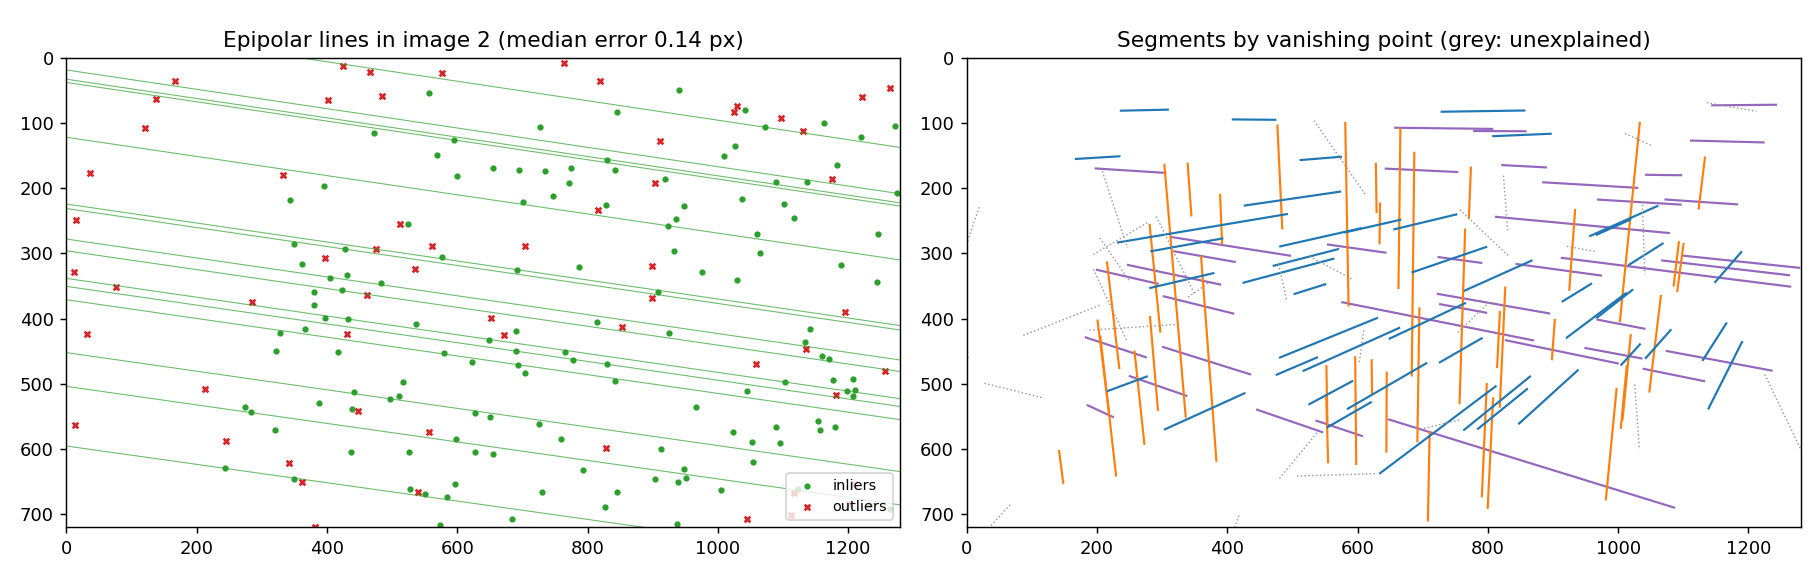
\includegraphics[width=0.85\linewidth]{geometry_synthetic.png}
\caption{Vérification synthétique de $F$ et des points de fuite (\texttt{python -m src.geometry.demo}).}
\end{figure}

\begin{resultat}
\textbf{Nos scènes} (erreur trois vues en px, écart 5 / écart 24, et croissance) :
\begin{center}\small
\resizebox{\linewidth}{!}{\begin{tabular}{llccc}
\toprule
Scène & Clip & Erreur (px) & Croissance & Sampson gén./réel \\
\midrule
aérien & réel / généré & 0,34 / 0,70 \quad 0,21 / 0,43 & 2,06 / 2,07 & 0,67 \\
chemin & réel / gén. 1 / gén. 2 & 0,38 / 0,50 \quad 0,49 / 0,54 \quad 0,48 / 0,55 & 1,30 / 1,10 / 1,15 & 1,33 / 1,31 \\
passerelle & réel / Omni / Seedance 2 & 0,64 / 1,09 \quad 0,64 / 1,09 \quad 0,52 / 0,87 & 1,70 / 1,70 / 1,68 & 1,70 / 1,56 \\
rugby & réel / généré & 0,94 / 0,88 \quad 0,32 / 0,39 & 0,94 / 1,21 & 0,74 \\
rue (écart 12) & réel / généré & 0,91 / 0,84 \quad 0,88 / 0,90 & 0,92 / 1,03 & 1,52 \\
drone & réel / généré & 0,29 / 0,47 \quad 0,37 / 0,70 & 1,62 / 1,90 & 1,06 \\
\bottomrule
\end{tabular}}
\end{center}
Seul le drone (vid6, forte parallaxe) montre une croissance nettement plus forte côté généré. Rugby et
rue ont des croissances inférieures à 1 côté réel : des passants bougent et les pistes longues
survivent moins.
\end{resultat}

\begin{figure}[!htbp]
\centering
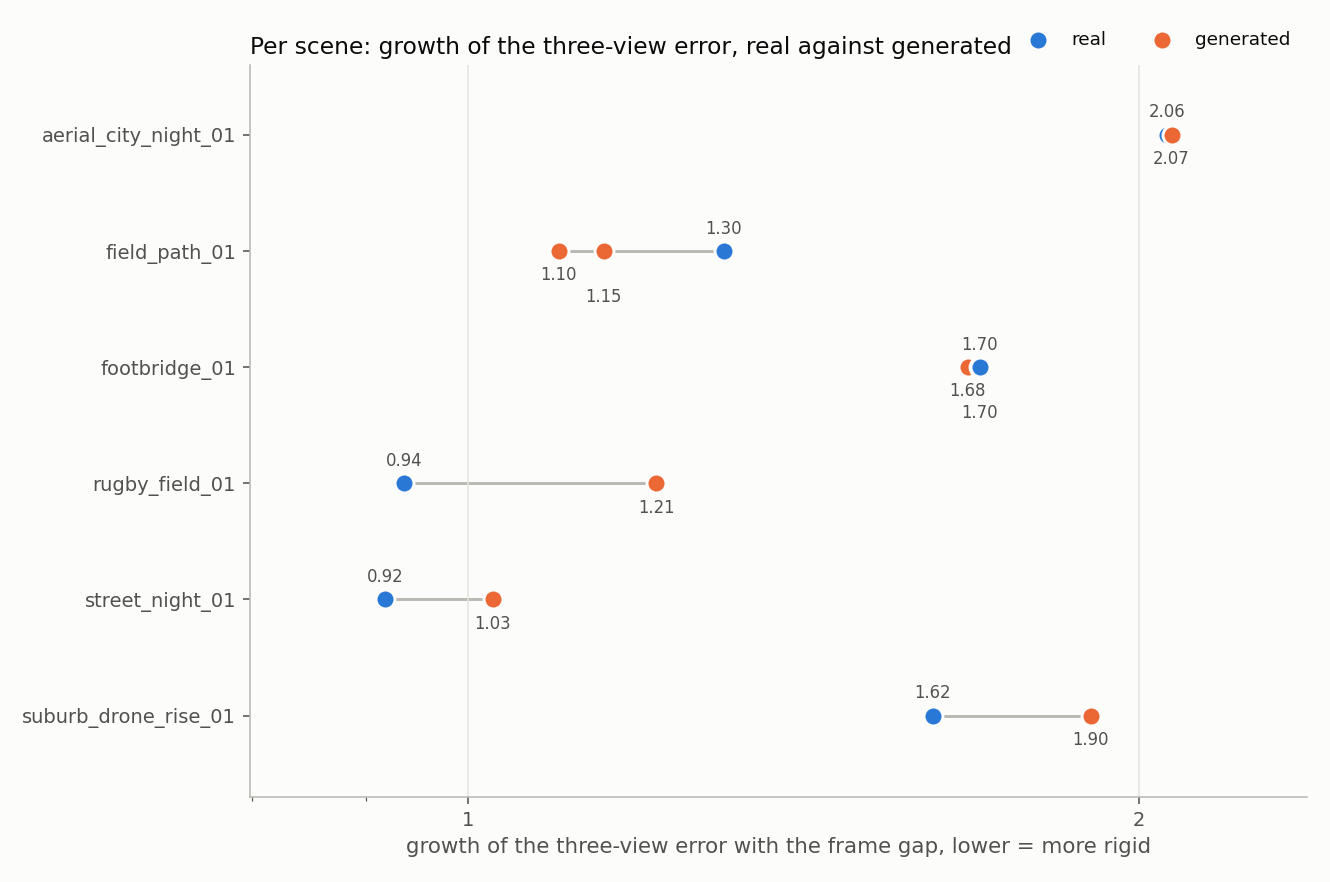
\includegraphics[width=0.8\linewidth]{v1_three_view_growth.png}
\caption{Erreur trois vues en fonction de l'écart, nos scènes.}
\end{figure}

\begin{piege}
\textbf{La croissance n'est invariante qu'à un rendu \emph{multiplicatif}.} Si l'erreur est
$e(k)=\sigma+\delta k$ (plancher de bruit $\sigma$ + dérive $\delta$ par frame), alors
$g=\frac{\sigma+\delta k_{\max}}{\sigma+\delta k_{\min}}$ dépend de $\sigma$ : à dérive égale, une vidéo
plus nette (petit $\sigma$) a une croissance plus grande. C'est exactement ce qui s'est passé sur
ViF-Bench (exercice 5 et section~\ref{sec:vif}).
\end{piege}

\subsection{Points de fuite dans le temps (I2, Sessions 1--4)}

\begin{intuition}
Les arêtes parallèles d'un bâtiment convergent vers un point de fuite. Ce point indique une
\emph{direction 3D}. Quand la caméra tourne, toutes les directions 3D de la scène tournent avec la
\emph{même} rotation. Une scène générée qui se déforme fait tourner ses directions de façon
incohérente.
\end{intuition}

\paragraph{Formalisme} (\texttt{src/geometry/vanishing.py}, \texttt{src/features/image\_perspective.py}).
\begin{enumerate}
  \item Segments par LSD, gardés si longueur $\ge$ 4\,\% de la diagonale.
  \item Chaque segment donne une droite $\boldsymbol\ell=\mathbf p_1\times\mathbf p_2$. Hypothèse de
        point de fuite $\mathbf v=\boldsymbol\ell_1\times\boldsymbol\ell_2$ (échantillon minimal $s=2$).
  \item Résidu angulaire : angle entre le segment et la droite qui joint son milieu $\mathbf m$ à
        $\mathbf v$ ; direction $\mathbf v_{1:2}-v_3\,\mathbf m$, valable même si $\mathbf v$ est à
        l'infini ($v_3=0$). Inlier si angle $<2^\circ$.
  \item Raffinement : $\min_{\|\mathbf v\|=1}\sum_i w_i(\boldsymbol\ell_i\T\mathbf v)^2$ par SVD.
        RANSAC séquentiel : on retire les inliers et on recommence (jusqu'à 3 points de fuite).
  \item Direction 3D : $\mathbf d=K^{-1}\mathbf v$ normalisée, avec une focale \textbf{supposée}
        $f=0{,}8\times$ le plus grand côté.
  \item Rotation commune entre deux frames par Procrustes orthogonal :
        $R=\arg\min\sum\|R\mathbf a_k-\mathbf b_k\|^2$, $R=U\,\mathrm{diag}(1,1,\det(UV\T))\,V\T$ avec
        $U\Sigma V\T=\mathrm{SVD}(B\T A)$. Le résidu angulaire après cette rotation
        (\texttt{i2\_rot\_resid\_deg}) est l'indice : une caméra qui tremble ne le change pas.
\end{enumerate}

\begin{exemple}
Image $1280\times720$, $f=0{,}8\times1280=1024$, $(c_x,c_y)=(640,360)$, point de fuite
$\mathbf v=(1664,360,1)$. $K^{-1}\mathbf v=\bigl((1664-640)/1024,\ 0,\ 1\bigr)=(1,0,1)$ : direction à
$45^\circ$ de l'axe optique, dans le plan horizontal.
\end{exemple}

\begin{resultat}
Drone vid6 : résidu de rotation $0{,}64^\circ$ (réel) contre $0{,}98^\circ$ (généré) ; variation de
l'angle entre deux directions $0{,}49^\circ$ contre $1{,}22^\circ$. Cohérent avec la croissance trois
vues plus forte du généré.
\end{resultat}

\begin{piege}
\begin{itemize}
  \item Ne s'applique qu'aux scènes avec des lignes droites (bâtiments, routes). Sans lignes : pas de
        mesure, pas \og vidéo réelle \fg.
  \item La focale est supposée : les angles absolus (orthogonalité) sont faux de quelques degrés, mais
        l'erreur est lisse dans le temps ; ce sont les \emph{variations} qui comptent.
  \item Le jitter d'une direction mélange tremblement de caméra et instabilité de la scène ; seul le
        résidu après rotation commune isole la scène.
\end{itemize}
\end{piege}

\subsection{Cohérence temporelle par flot optique (V3, Sessions 3 et 6)}

\begin{intuition}
Si l'on compense le mouvement, la frame suivante doit retomber sur la frame courante, au bruit près.
Les vidéos générées \og bouillonnent \fg{} parfois : la texture fine change même là où rien ne bouge.
\end{intuition}

\paragraph{Formalisme} (\texttt{src/features/video\_temporal.py}).
Flot dense de Farnebäck aller $\mathbf f$ et retour $\mathbf b$. Un pixel est gardé si
\[ \|\mathbf f(\x)+\mathbf b(\x+\mathbf f(\x))\| < 0{,}5+0{,}05\,\|\mathbf f(\x)\| \]
(test aller-retour : élimine occlusions et échecs du flot ; la tolérance grandit avec le mouvement).
On recale $I_{t+1}$ sur $I_t$ et on mesure le résidu, sur l'image, sur sa partie haute fréquence
$I-G_{1{,}5}*I$, et sur les pixels quasi immobiles.

\begin{resultat}
ViF-Bench : AUC 0,49 (hasard). Vérification : sur ces clips de 256 px, la \emph{médiane} du résidu et du
flot vaut souvent exactement 0, et les clips contiennent des frames dupliquées. Version corrigée
(pixels texturés, moyenne, frames dupliquées ignorées) sur 40 scènes : AUC 0,52 ; par générateur, les
rapports généré/réel vont dans les deux sens (SkyReels 0,69, gen4 0,67, Wan2.2-TI2V-T 1,50). V3 mesure
une signature de rendu propre à chaque générateur, pas une loi universelle.
\end{resultat}

\subsection{Spectre du bruit (I1, Sessions 1--2)}

\begin{intuition}
Les générateurs agrandissent des images par des couches de suréchantillonnage, qui laissent des
motifs périodiques invisibles à l'\oe il mais visibles comme des pics dans le spectre de Fourier du
\emph{bruit}.
\end{intuition}

\paragraph{Formalisme} (\texttt{src/features/image\_frequency.py}).
Résidu $r=I-\mathrm{med}_{3\times3}(I)$ (le filtre médian enlève la scène, garde le bruit) ; fenêtre de
Hann $w$ (évite les fuites spectrales des bords) ; $P=\log_{10}|\mathcal F(r\,w)|^2$ moyenné sur 16
frames (les pics périodiques s'additionnent, le bruit aléatoire se moyenne) ; profil radial (moyenne
de $P$ sur des anneaux de fréquence) ; excès de chaque fréquence sur la moyenne de son anneau
(\texttt{i1\_peak\_max}) ; part d'énergie au-delà de $0{,}25$ cycle/pixel.

\begin{resultat}
ViF-Bench : AUC 0,56. Les vidéos sont réduites, ré-encodées en H.264 : la compression et le
redimensionnement effacent l'essentiel des traces de suréchantillonnage.
\end{resultat}

\subsection{Classification et évaluation (Session 5)}

\begin{intuition}
Chaque vidéo devient un vecteur de mesures. Un classifieur simple apprend à séparer réel et généré.
La question n'est pas \og quel score maximal \fg{} mais \og quelle famille de mesures porte de
l'information, et est-ce de la physique ou autre chose \fg.
\end{intuition}

\paragraph{Formalisme} (\texttt{src/models/classify.py}).
\begin{itemize}
  \item Familles physiques : gradient boosting (gère les valeurs manquantes). CLIP : régression
        logistique sur les 512 dimensions de ViT-B/32 moyennées sur 8 frames (linear probe, UnivFD).
  \item Validation croisée à 5 plis \textbf{groupés par scène} : un clip réel et toutes ses versions
        générées sont dans le même pli.
  \item AUC sur les scores hors-pli, intervalle de confiance par bootstrap sur les scènes.
  \item Générateur jamais vu : on retire un générateur de l'apprentissage, on le teste seul.
\end{itemize}

\begin{resultat}
\begin{center}\small
\begin{tabular}{lccc}
\toprule
Famille & AUC [IC 95\,\%] & Générateur jamais vu (moyenne) \\
\midrule
V1 géométrie & 0,62 [0,58 ; 0,67] & 0,60 \\
I1 fréquence & 0,56 & -- \\
V3 temporel & 0,49 & -- \\
physique (V1+I1+V3) & 0,65 [0,61 ; 0,69] & 0,62 \\
CLIP & 0,77 [0,74 ; 0,80] & 0,75 \\
physique + CLIP (concaténation) & 0,77 & 0,74 \\
fusion tardive (rangs, poids 0,25 physique) & 0,786 & -- \\
\bottomrule
\end{tabular}
\end{center}
Gain de la fusion tardive sur CLIP : +0,018 [0,008 ; 0,030] (500 bootstraps par scène). Le poids a été
choisi sur les mêmes données, donc ce gain est légèrement optimiste (avec un poids de 0,35 :
+0,017 [0,001 ; 0,033]).

\textbf{Mouvement ou cohérence 3D ?} Les features de mouvement seules donnent 0,59. Ajouter la
cohérence 3D au mouvement apporte $-0{,}0005$ sur tous les générateurs, mais +0,044 [0,010 ; 0,078] sur
les générateurs image-to-video. La cohérence corrigée du mouvement donne 0,62.
\end{resultat}

\begin{piege}
\begin{itemize}
  \item \textbf{Exactitude équilibrée 0,52 avec une AUC 0,65} : les scores sont tous au-dessus de 0,8
        (95\,\% des vidéos sont générées), le seuil 0,5 n'a aucun sens. Seule l'AUC compte.
  \item \textbf{Concaténer} 115 features physiques et 512 de CLIP dans une régression logistique :
        CLIP domine. La fusion tardive des scores révèle la petite complémentarité.
  \item \textbf{Découper par fichier} au lieu de par scène : le modèle reconnaît le contenu de la scène.
\end{itemize}
\end{piege}

\subsection{ViF-Bench : le confondant du plancher de bruit}\label{sec:vif}

ViF-Bench : 165 clips réels, 19 générateurs, 3160 vidéos, 256 px de haut, 16 fps, 5 s.

\begin{resultat}
\textbf{Première lecture} (encore dans le rapport actuel) : croissance trois vues générée/réelle 1,08
en médiane, générée plus grande dans 58\,\% des paires (Wilcoxon $p=0{,}002$), HunyuanVideo-I2V 1,30,
LTX-T 1,29, sora-2 1,18.

\textbf{Vérification} :
\begin{itemize}
  \item le rapport des croissances suit le rapport des planchers d'erreur à l'écart 3 (Spearman
        $-0{,}21$, $p=10^{-25}$) et, entre générateurs, le rapport de mouvement ($-0{,}56$, $p=0{,}01$) ;
  \item paires à mouvement comparable (353) : médiane 1,002, $p=0{,}61$ ;
  \item après régression sur log(mouvement) et log(plancher) : médiane 1,004, $p=0{,}80$.
\end{itemize}
HunyuanVideo-I2V est le seul générateur en $928\times544$ à 24 fps : réduit d'un facteur 2,1, il est
plus net que les autres, donc son plancher est plus bas et sa croissance plus haute.

\textbf{Conclusion correcte} : sur ViF-Bench, nous ne détectons pas de dérive 3D des vidéos générées à
mouvement et précision égaux.
\end{resultat}

Autres biais du benchmark (scan de toutes les vidéos, \texttt{results/vifbench\_frame\_scan.csv}) :
5,5\,\% des clips réels sont statiques ; les clips réels contiennent des frames dupliquées irrégulières
(frame rate variable) ; 22\,\% des clips CogVideoX sont statiques.

\subsection{V5 (hors cours) : le flot est-il celui d'une caméra ?}

\begin{intuition}
Si l'on connaît la profondeur de chaque pixel, le mouvement de tous les pixels est dicté par six
nombres seulement : la vitesse de translation et de rotation de la caméra. Un réseau de neurones
(Depth Anything V2) estime la profondeur dans une seule image. On cherche les six nombres qui
expliquent au mieux le flot observé ; ce qui reste inexpliqué, c'est ce qui n'est pas une caméra
dans une scène rigide : objets mobiles, ou scène générée dont le mouvement ne suit pas sa propre
profondeur.
\end{intuition}

\paragraph{Formalisme} (Longuet-Higgins et Prazdny 1980 ; Szeliski ch. 9, 11, 12 ;
\texttt{src/features/video\_rigidflow.py}). Coordonnées normalisées $x=(u-c_x)/f$, $y=(v-c_y)/f$,
profondeur inverse $\rho=1/Z$, translation $\mathbf t$, rotation $\boldsymbol\omega$ :
\[
\begin{aligned}
\dot u &= \rho\,(-t_x + x\,t_z) \;+\; x y\,\omega_x - (1+x^2)\,\omega_y + y\,\omega_z,\\
\dot v &= \rho\,(-t_y + y\,t_z) \;+\; (1+y^2)\,\omega_x - x y\,\omega_y - x\,\omega_z .
\end{aligned}
\]
Rôle des termes :
\begin{itemize}
  \item \textbf{partie translation} $\rho(\cdot)$ : proportionnelle à $\rho$ ; un objet proche (grand
        $\rho$) bouge plus. C'est la parallaxe. $t_z$ (avancer) crée un flot radial depuis le centre ;
  \item \textbf{partie rotation} : indépendante de la profondeur. Si $\mathbf t=0$, la profondeur ne
        sert à rien (cas dégénéré, comme l'homographie pour $F$) ;
  \item le réseau donne $d$ à une échelle et un décalage près : $\rho=a\,d+b$. En développant,
        $\rho\,\mathbf t = d\,(a\mathbf t) + b\mathbf t$ : le modèle est \textbf{linéaire} en 9 inconnues
        $(a\mathbf t,\ b\mathbf t,\ \boldsymbol\omega)$.
\end{itemize}
Résolution : moindres carrés repondérés (IRLS, poids de type Cauchy : un pixel loin du modèle pèse
peu) sur les pixels texturés qui passent le test aller-retour. Résidu par pixel en px. Features :
résidu médian \texttt{v5\_res\_px}, part de pixels au-delà de 1 px \texttt{v5\_bad\_frac}, résidu du
modèle rotation seule (3 inconnues) et le rapport des deux \texttt{v5\_gain} (ce que la profondeur explique).

\begin{exemple}
Frames $640\times360$, $f=0{,}8\times640=512$. Point $x=0{,}1$, $y=0$.
\begin{itemize}
  \item Rotation $\omega_y=0{,}01$ seule : $\dot u=-(1+0{,}01)\times0{,}01=-0{,}0101$, soit
        $-0{,}0101\times512=-5{,}2$ px, \emph{quelle que soit la profondeur}.
  \item Translation $t_x=0{,}05$ seule : $\dot u=-0{,}05\,\rho$. Pour $\rho=0{,}5$ : $-12{,}8$ px ; pour
        $\rho=0{,}25$ (deux fois plus loin) : $-6{,}4$ px. La profondeur règle l'amplitude.
\end{itemize}
\end{exemple}

\begin{resultat}
\begin{itemize}
  \item Tests (\texttt{tests/test\_rigidflow.py}, 6 tests) : flot rigide exact retrouvé à $10^{-6}$ px ;
        invariance à l'échelle et au décalage de la profondeur ; un objet mobile ressort ($>2$ px) sans
        perturber le fond ($<0{,}05$ px).
  \item Synthétique, écart 8 frames : propre 0,385 px, flou 0,378 px, dérive 4 px 0,484 px (+26\,\%).
        Même comportement que le test à trois vues : sensible à la dérive, pas au flou.
  \item Drone vid6 : 0,57 px (réel) contre 0,97 px (généré) ; 15\,\% contre 48\,\% de pixels hors modèle.
  \item Autres scènes : pas de sens constant (passerelle 2,16 réel contre 1,08 et 0,81 générés ; rugby
        6,65 contre 0,11, car le réel contient des joueurs qui bougent).
  \item Sur ViF-Bench : calcul commencé (153 vidéos sur 732), interrompu par manque de RAM. Pas encore
        de chiffre.
\end{itemize}
\end{resultat}

\begin{figure}[!htbp]
\centering
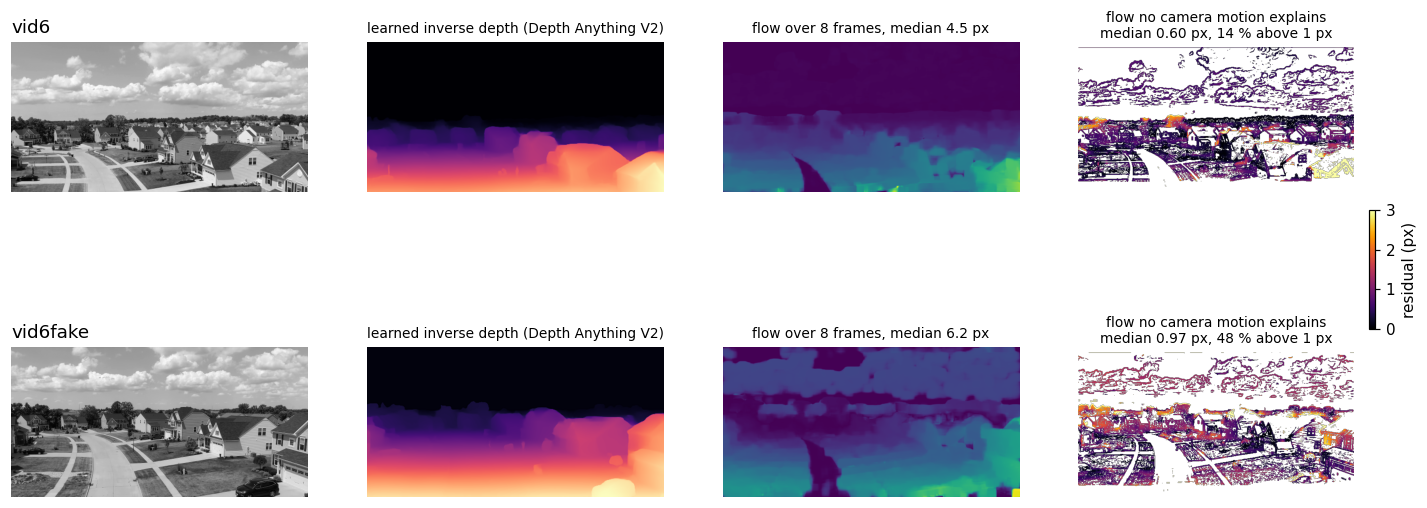
\includegraphics[width=\linewidth]{v5_residual_vid6.png}
\caption{V5 sur le drone : frame, profondeur inverse apprise, flot sur 8 frames, et carte du flot
qu'aucun mouvement de caméra n'explique. Le généré a beaucoup plus de pixels au-delà de 1 px.}
\end{figure}

\begin{piege}
\begin{itemize}
  \item Le résidu monte aussi pour de \textbf{vrais} objets mobiles : V5 ne dit pas \og faux \fg, il dit
        \og pas une caméra dans une scène rigide \fg. La carte montre \emph{où}.
  \item La focale est supposée ; la profondeur du réseau peut être fausse sur le ciel ou les reflets.
        Le fit robuste limite l'effet, sans l'annuler.
  \item Le réseau est \emph{appris} : c'est un a priori extérieur, pas une mesure. C'est pour cela que
        V5 est présenté comme hors cours, à côté des méthodes implémentées de bout en bout.
\end{itemize}
\end{piege}

\subsection{Données et normalisation}
\begin{itemize}
  \item Nos clips : 6 réels, 10 générés (8 appariés par image-to-video à partir de la première frame du
        réel, 2 non appariés). Scènes statiques avec structures (routes, passerelle, drone).
  \item Même traitement pour tous : 24 fps, petit côté 720 px, H.264 CRF 18, 0,5 s sautées au début
        (la première frame d'un image-to-video est réelle), 10\,\% du bas recadrés (filigranes).
  \item \texttt{data/raw/} n'est jamais modifié ; tout va dans \texttt{data/processed/}.
\end{itemize}

%=====================================================================================
\section{Méthodologie et boîte à outils}
%=====================================================================================

\subsection{Guide réflexe : face à telle question, quelle méthode ?}

\begin{center}\small
\begin{tabular}{p{6.3cm}p{8.7cm}}
\toprule
Situation ou question & Méthode et raison \\
\midrule
La caméra translate dans une scène statique & V1 : $F$ par RANSAC, Sampson. Contrainte de base. \\
\texttt{h\_cover} proche de 1, parallaxe faible & Rotation pure ou scène lointaine : $F$ non informative. Regarder $H$, I2, V5 rotation. \\
Un point peut glisser le long de sa droite & Test à trois vues (Session 7) : contrainte de point. \\
Le généré est plus flou ou plus net & Comparer des \emph{croissances} ou des résidus normalisés, jamais Sampson brut ; vérifier avec un contrôle (fenêtre copiée, flou synthétique). \\
Le généré bouge moins & Comparer à mouvement image égal (intervalles de flot communs). \\
Scène urbaine avec lignes & I2 : points de fuite, résidu après rotation commune. \\
Caméra fixe, rien ne bouge & V1, V3 et V5 ne s'appliquent pas ; seul I1 (et CLIP). \\
Où dans l'image le modèle de caméra casse-t-il ? & V5 : carte du résidu par pixel. \\
Une feature sépare bien réel et généré & Se demander si c'est du mouvement, du rendu ou du contenu ; tester à mouvement égal ; regarder par générateur. \\
Évaluer un classifieur & AUC hors-pli, CV groupée par scène, IC par bootstrap sur scènes, générateur jamais vu. \\
\bottomrule
\end{tabular}
\end{center}

\subsection{Recette : analyser une paire réel / généré}
\begin{enumerate}
  \item Normaliser les deux clips de la même façon ; sauter la fenêtre de conditionnement.
  \item Vérifier qu'il y a du mouvement \emph{et} de la parallaxe (sinon : pas de test 3D).
  \item Mesurer V1 à plusieurs écarts ; comparer Sampson à mouvement égal.
  \item Mesurer la croissance trois vues sur les mêmes écarts ; comparer aussi le plancher
        $e(k_{\min})$ : si les planchers diffèrent beaucoup, la croissance n'est pas comparable.
  \item Compléter par I2 (si lignes) et V5 (carte du résidu).
  \item Conclure seulement si plusieurs instruments indépendants vont dans le même sens (vid6 : trois vues,
        I2 et V5 d'accord).
\end{enumerate}
Commande : \texttt{python -m src.eval.inspect\_video réel.mp4 généré.mp4}.

\subsection{Recette : vérifier qu'un instrument mesure ce qu'on croit}
\begin{enumerate}
  \item Clip synthétique de géométrie connue (\texttt{src/geometry/synth\_video.py}).
  \item Trois versions : propre, rendu dégradé (flou, bruit), scène qui dérive.
  \item Un bon instrument géométrique : insensible à la deuxième, sensible à la troisième.
\end{enumerate}

%=====================================================================================
\section{Exercices corrigés}
%=====================================================================================

\subsection*{Exercice 1 (application directe) : distance de Sampson}
Avec $F=\begin{pmatrix}0&0&0\\0&0&-1\\0&1&0\end{pmatrix}$, calculer $d_S$ pour $\x=(200,80)$ et
$\x'=(260,83)$. L'appariement est-il inlier au seuil de 1,5 px ? Que représente ce $F$ ?

\paragraph{Correction.}
$F\x=(0,\,-1,\,80)\T$ ; $\x^{\prime\mathsf{T}} F\x=0\cdot260+(-1)\cdot83+80=-3$, donc numérateur 3.
$F\T\x'=(0,\,1,\,-83)\T$. Dénominateur $\sqrt{0^2+(-1)^2+0^2+1^2}=\sqrt2$.
$d_S=3/\sqrt2=2{,}12$ px : \textbf{outlier} ($>1{,}5$ px). Ce $F$ code une translation horizontale
pure (droites épipolaires horizontales : $v'=v$). Le point a bougé de 3 px verticalement, ce qu'une
telle caméra ne peut pas produire pour un point immobile. Le facteur $\sqrt2$ vient du partage de
la correction entre les deux points.

\subsection*{Exercice 2 (application) : nombre de tirages RANSAC}
Avec $p=0{,}99$, calculer $N$ pour : (a) $F$, $e=0{,}3$ ; (b) caméra par DLT, $e=0{,}3$ ; (c) point
de fuite, $e=0{,}5$. Pourquoi le DLT de caméra utilise-t-il 6 points ?

\paragraph{Correction.}
(a) $s=8$ : $0{,}7^8=0{,}0576$, $N=\lceil-4{,}605/\log(0{,}9424)\rceil=\lceil77{,}6\rceil=78$.
(b) $s=6$ : $0{,}7^6=0{,}1176$, $\log(0{,}8824)=-0{,}1251$, $N=\lceil36{,}8\rceil=37$.
(c) $s=2$ : $0{,}5^2=0{,}25$, $\log(0{,}75)=-0{,}2877$, $N=\lceil16{,}01\rceil=17$.
Une caméra $3\times4$ a 12 coefficients à l'échelle près, soit 11 degrés de liberté ; chaque
correspondance 3D--2D donne 2 équations ; il faut donc $\lceil11/2\rceil=6$ points.

\subsection*{Exercice 3 (compréhension) : point de fuite et rotation}
Image $1280\times720$, focale supposée $1024$, point principal au centre. Dans la frame $t$, deux points
de fuite sont $\mathbf v_1=(1664,360,1)$ et $\mathbf v_2=(640,-664,1)$. (a) Calculer les directions 3D.
(b) Quel angle forment-elles ? (c) Dans la frame $t+1$, la caméra a tourné ; pourquoi l'angle entre les
deux directions doit-il rester le même pour une vraie caméra ?

\paragraph{Correction.}
(a) $K^{-1}\mathbf v_1=(1,0,1)$, normalisé $(0{,}707,0,0{,}707)$ ;
$K^{-1}\mathbf v_2=\bigl(0,(-664-360)/1024,1\bigr)=(0,-1,1)$, normalisé $(0,-0{,}707,0{,}707)$.
(b) Produit scalaire $0{,}5$, donc $60^\circ$ (le signe d'une direction est libre ; on prend l'angle
entre 0 et $90^\circ$).
(c) Les directions sont celles d'arêtes fixes de la scène, exprimées dans le repère de la caméra. Une
rotation $R$ de la caméra les transforme toutes en $R\mathbf d$, et une rotation conserve les angles.
Si l'angle varie (au-delà du bruit et de l'erreur lisse due à la focale supposée), la scène elle-même
se déforme. C'est la feature \texttt{i2\_pair\_angle\_std\_deg}.

\subsection*{Exercice 4 (V5) : linéarité et dégénérescence}
(a) Montrer que, si $\rho=a\,d+b$ avec $a,b$ inconnus, le flot rigide est linéaire en 9 paramètres.
(b) Pourquoi la profondeur ne sert-elle à rien si la caméra ne fait que tourner ? (c) Que vaut
\texttt{v5\_gain} dans ce cas ?

\paragraph{Correction.}
(a) La partie translation s'écrit $\rho(-t_x+x t_z)=d\,(-at_x+x\,at_z)+(-bt_x+x\,bt_z)$. En posant
$\boldsymbol\alpha=a\mathbf t$ et $\boldsymbol\beta=b\mathbf t$, chaque composante du flot est une
combinaison linéaire de $\boldsymbol\alpha$ (coefficients dépendant de $d,x,y$), de $\boldsymbol\beta$
(coefficients dépendant de $x,y$) et de $\boldsymbol\omega$ : 3+3+3 = 9 inconnues, système linéaire.
(b) Avec $\mathbf t=0$, $\boldsymbol\alpha=\boldsymbol\beta=0$ et le flot ne contient que la partie
rotation, qui ne dépend pas de $\rho$. Comme pour $F$ face à une homographie, la 3D n'est pas observable.
(c) Les deux modèles (rotation seule et avec profondeur) expliquent le flot aussi bien : résidus
égaux, \texttt{v5\_gain} $\approx1$. Un gain élevé (vid1 : 13,7) indique au contraire une forte
parallaxe, là où le test est le plus informatif.

\subsection*{Exercice 5 (piège A+) : la croissance trompeuse}
L'erreur trois vues suit $e(k)=\sigma+\delta k$. Vidéo réelle : $\sigma=0{,}25$ px,
$\delta=0{,}002$ px/frame. Vidéo générée : \emph{même dérive} $\delta$, mais plus nette,
$\sigma=0{,}15$ px. Écarts $k_{\min}=3$, $k_{\max}=16$. (a) Calculer les deux croissances.
(b) Qu'aurait conclu un analyste naïf ? (c) Quel protocole évite l'erreur ?

\paragraph{Correction.}
(a) Réel : $e(3)=0{,}256$, $e(16)=0{,}282$, $g=1{,}10$. Généré : $e(3)=0{,}156$, $e(16)=0{,}182$,
$g=1{,}17$.
(b) \og La vidéo générée dérive davantage \fg, alors que la dérive est identique : seule la netteté
diffère. La croissance n'est invariante qu'à un facteur multiplicatif, pas à un plancher additif.
(c) Estimer directement la pente $\delta$ (différence $e(k_{\max})-e(k_{\min})$ divisée par
$k_{\max}-k_{\min}$, ici $0{,}002$ des deux côtés), ou comparer des vidéos de plancher et de mouvement
égaux, ou régresser le rapport de croissance sur le rapport des planchers et du mouvement. C'est ce qui
a fait disparaître l'effet sur ViF-Bench (médiane 1,004, $p=0{,}80$). Attention : la différence est
sensible au mouvement, il faut donc aussi comparer à mouvement égal.

\subsection*{Exercice 6 (piège A+) : interpréter un contrôle et une évaluation}
(a) Sur vid4, le rapport de Sampson généré/réel vaut 1,31 sur tout le clip et 1,29 dans les 2 premières
secondes, recopiées du réel par le générateur. Que peut-on conclure ? (b) Un classifieur a une AUC de
0,65 mais une exactitude équilibrée de 0,52. Est-ce contradictoire ? (c) Si l'on découpe la validation
croisée par fichier, que se passe-t-il ?

\paragraph{Correction.}
(a) Dans la fenêtre copiée, la géométrie est vraie par construction. Un écart de 1,29 y existe quand
même : il ne peut venir que du rendu (texture, netteté, localisation des points SIFT). Comme l'écart est
le même ensuite, rien n'indique une erreur 3D supplémentaire : Sampson brut n'est pas une mesure de 3D.
(b) Non. L'AUC mesure le classement des scores, indépendamment du seuil. Avec 95\,\% de vidéos générées,
le classifieur donne des scores tous élevés ; au seuil 0,5, presque tout est \og généré \fg{} et
l'exactitude équilibrée est proche de 0,5. Le classement reste pourtant meilleur que le hasard.
(c) Une scène et ses versions générées partagent le contenu (même rue, même ciel). Le modèle
apprendrait à reconnaître la scène et son jumeau, pas un indice physique : l'AUC serait gonflée et
ne généraliserait pas.

%=====================================================================================
\section{Fiche synthèse et auto-évaluation}
%=====================================================================================

\subsection{Cheat sheet}
\begin{center}\small
\begin{tabular}{p{4.2cm}p{10.8cm}}
\toprule
Notion & Formule ou règle \\
\midrule
Projection & $\lambda\x=K[R|t]\X$ ; droite $\boldsymbol\ell=\x_1\times\x_2$ ; intersection $\boldsymbol\ell_1\times\boldsymbol\ell_2$ \\
RANSAC & $N=\log(1-p)/\log(1-(1-e)^s)$ ; $s$ = 8 ($F$), 4 ($H$), 6 (caméra), 2 (point de fuite) \\
Épipolaire & $\x^{\prime\mathsf{T}} F\x=0$ ; rang 2 ; 7 ddl ; 8 points normalisé, $F=T^{\prime\mathsf{T}}\hat FT$ \\
Sampson & $|\x^{\prime\mathsf{T}} F\x|/\sqrt{(F\x)_1^2+(F\x)_2^2+(F\T\x')_1^2+(F\T\x')_2^2}$ (px) \\
Homographie & $\x'\sim H\x$, 8 ddl ; \texttt{h\_cover}, parallaxe = ce que $H$ n'explique pas \\
Caméras depuis $F$ & $P_1=[I|0]$, $P_2=[[\mathbf e']_\times F\,|\,\mathbf e']$, $F\T\mathbf e'=0$ \\
Triangulation & $(x\mathbf p_3\T-\mathbf p_1\T)\X=0$, $(y\mathbf p_3\T-\mathbf p_2\T)\X=0$, SVD \\
DLT de caméra & 11 ddl, 2 éq./point, $\ge6$ points \\
Croissance & $g=e(k_{\max})/e(k_{\min})$ : invariante à un facteur, pas à un plancher additif \\
Point de fuite & $\mathbf v=\boldsymbol\ell_1\times\boldsymbol\ell_2$ ; $\mathbf d=K^{-1}\mathbf v$ ; Procrustes $R=U\,\mathrm{diag}(1,1,\det UV\T)V\T$ \\
Test aller-retour & $\|\mathbf f+\mathbf b(\x+\mathbf f)\|<0{,}5+0{,}05\|\mathbf f\|$ \\
I1 & $r=I-\mathrm{med}_3(I)$, $\log_{10}|\mathcal F(rw)|^2$, profil radial, excès sur l'anneau \\
V5 & $\dot u=\rho(-t_x+xt_z)+xy\omega_x-(1+x^2)\omega_y+y\omega_z$ ; $\rho=ad+b$ $\Rightarrow$ 9 inconnues linéaires \\
Évaluation & AUC hors-pli, CV groupée par scène, bootstrap par scène, générateur jamais vu \\
Confondants & rendu (flou, netteté), mouvement, plancher de bruit, objets mobiles, frames dupliquées \\
\bottomrule
\end{tabular}
\end{center}

\subsection{Chiffres clés}
\begin{itemize}[nosep]
  \item Synthétique : croissance 1,44 (propre), 1,41 (flou), 3,24 (dérive) ; V5 +26\,\% sous dérive.
  \item vid4 : Sampson généré/réel 1,30 et 1,29 dans la fenêtre copiée (rendu).
  \item vid6 : croissance 1,62 / 1,90 ; I2 $0{,}64^\circ$ / $0{,}98^\circ$ ; V5 0,57 / 0,97 px.
  \item ViF-Bench : physique 0,65, CLIP 0,77, fusion tardive 0,786 ; croissance corrigée 1,004 ($p=0{,}80$).
  \item 85 tests unitaires passent.
\end{itemize}

\subsection{Dix questions de contrôle}
\begin{enumerate}
  \item Pourquoi faut-il normaliser les coordonnées avant l'algorithme des 8 points ?
  \item Pourquoi force-t-on le rang 2 de $F$, et comment ?
  \item Qu'est-ce que le contrôle de la fenêtre copiée de vid4 a démontré ?
  \item Pourquoi compare-t-on à mouvement égal et non à écart temporel égal ?
  \item Pourquoi le test à trois vues n'a-t-il pas besoin de la calibration $K$ ?
  \item Dans quel cas la croissance trois vues est-elle trompeuse ?
  \item Quelle quantité I2 est insensible au tremblement de la caméra, et pourquoi ?
  \item Pourquoi V3 donnait-il une AUC de 0,49 sur ViF-Bench ?
  \item Pourquoi V5 a-t-il 9 inconnues et non 6 ?
  \item Pourquoi la concaténation physique + CLIP n'apporte-t-elle rien alors que la fusion tardive aide ?
\end{enumerate}

\newpage
\subsection*{Réponses}
\begin{enumerate}
  \item Les colonnes de la matrice $A$ ont des ordres de grandeur très différents ($uu'\sim10^6$ contre
        1) ; la SVD est alors dominée par les grandes colonnes et le résultat est instable. Ramener les
        points vers $[-1,1]$ équilibre le système (Hartley 1997).
  \item Toute vraie $F$ est singulière : toutes les droites épipolaires passent par l'épipole. La
        solution de la SVD ne l'est pas à cause du bruit ; on annule la plus petite valeur singulière
        (projection au sens de Frobenius).
  \item Que l'écart de Sampson entre réel et généré (1,30) existe là où la géométrie est recopiée du
        réel : il vient du rendu, pas de la 3D.
  \item Toutes les erreurs croissent avec le mouvement, et les vidéos générées bougent souvent moins ;
        à écart égal, elles paraîtraient injustement plus cohérentes.
  \item La reconstruction projective $(P_1,P_2)$ depuis $F$ est fausse à une transformation projective
        près, mais la caméra de la vue 3 est estimée dans le même repère : les positions reprojetées
        dans l'image, seules comparées, n'en dépendent pas.
  \item Quand les planchers d'erreur diffèrent (netteté différente) : avec $e=\sigma+\delta k$, un
        $\sigma$ plus petit donne une croissance plus grande à dérive égale. Le mouvement joue aussi.
  \item Le résidu angulaire après la meilleure rotation commune (Procrustes) : une rotation de caméra,
        même saccadée, fait tourner toutes les directions ensemble et ne laisse aucun résidu.
  \item À 256 px, les médianes du résidu et du flot valaient souvent exactement 0, et des frames
        dupliquées donnaient des paires sans mouvement. Même corrigé, V3 reste à 0,52 : signature de
        rendu propre à chaque générateur.
  \item La profondeur du réseau est connue à une échelle $a$ et un décalage $b$ près. Les produits
        $a\mathbf t$ et $b\mathbf t$ remplacent $\mathbf t$ : 3+3 inconnues de translation + 3 de rotation.
  \item Dans une seule régression logistique, les 512 dimensions de CLIP dominent les 115 features
        physiques. En combinant les scores déjà appris séparément, chaque famille garde sa voix :
        +0,018 [0,008 ; 0,030].
\end{enumerate}

%=====================================================================================
\appendix
\section{État du projet et points ouverts (18 novembre 2026)}
\begin{itemize}
  \item Le rapport \texttt{main.tex} présente encore l'effet de croissance sur ViF-Bench comme un
        résultat, et dit que physique et CLIP ne se complètent pas. Ces deux passages sont à corriger
        (section~\ref{sec:vif} et fusion tardive).
  \item V3 sur ViF-Bench a été calculé avec une ancienne version (\texttt{v3\_static\_res\_med}) ; à
        recalculer avec le code corrigé.
  \item V5 sur ViF-Bench : à terminer (40 scènes, environ 12 min sur 4 processus) puis à évaluer.
  \item Le dossier local \texttt{results/latest\_vifbench} a été écrasé par un petit run de test ; la
        version complète est à recopier depuis la machine de l'école.
\end{itemize}

\end{document}
